
%(BEGIN_QUESTION)
% Copyright 2015, Tony R. Kuphaldt, released under the Creative Commons Attribution License (v 1.0)
% This means you may do almost anything with this work of mine, so long as you give me proper credit

Calculate the rate of liquid flow coming into process vessel V-5 at 1:30 PM, and also at 3:45 PM, based on the information shown here:

$$\includegraphics[width=15.5cm]{i02890x01.eps}$$

$Q_{in}$ @ 1:30 PM = \underbar{\hskip 50pt} GPM

\vskip 10pt

$Q_{in}$ @ 3:45 PM = \underbar{\hskip 50pt} GPM

\vskip 10pt

\underbar{file i02890}
%(END_QUESTION)





%(BEGIN_ANSWER)

At 1:30 PM, the level is increasing at a rate ($dV \over dt$) of 5 gallons per hour, which is equivalent to 0.083 GPM.  At that time the outgoing flow rate (FT-240) registers 35 GPM.  Therefore, the incoming flow rate must be 0.083 GPM greater than FT-240, which is 35.083 GPM.

\vskip 10pt

$Q_{in}$ @ 3:45 PM must be equal to $Q_{out}$ because the level (LT-31) is holding steady.  Therefore, $Q_{in}$ = 27.5 GPM at 3:45 PM.

\vskip 10pt

What this means is that the incoming flow decreased at the same time as the outgoing flow decreased (both at 2:00 PM).  Between Noon and 2:00 PM $Q_{in}$ was 35.083 GPM and $Q_{out}$ was 35 GPM, but then both flow rates stepped down to 27.5 GPM at 2:00 PM.

%(END_ANSWER)





%(BEGIN_NOTES)


%INDEX% Mathematics, calculus: integral (accumulated volume as the integral of flow)
%INDEX% Mathematics, calculus: integration (numerical)

%(END_NOTES)


